\documentclass[9pt]{beamer}
\usetheme{metropolis}
\usepackage{amsmath}
\usepackage{amssymb}
\usepackage{graphicx}
\usepackage{booktabs}
\usepackage{xcolor}
\usepackage{tikz}
\usetikzlibrary{arrows,positioning,shapes.geometric,calc}

% Define color palette matching our project design system
\definecolor{primary}{HTML}{1abc9c}    % Deep Teal
\definecolor{secondary}{HTML}{3498db}  % Astro Blue
\definecolor{darkbg}{HTML}{2c3e50}     % Slate Blue
\definecolor{accent}{HTML}{e67e22}     % Orange

\setbeamercolor{palette primary}{bg=darkbg, fg=white}
\setbeamercolor{palette secondary}{bg=primary, fg=white}
\setbeamercolor{palette tertiary}{bg=secondary, fg=white}
\setbeamercolor{structure}{fg=primary}
\setbeamercolor{alerted text}{fg=accent}

\title{Bayesian Statistics, MCMC, \& Physics-Informed Neural Networks}
\subtitle{Meet 3 Foundations: Parameter Uncertainty \& Constrained Machine Learning Models}
\author{Astronomy Club}
\date{\today}

\begin{document}

\maketitle

% Slide 2: Meet Overview
\begin{frame}{Meet Overview}
  This meet bridges the gap between statistical parameter estimation and machine learning by teaching Bayesian inference and Physics-Informed Neural Networks (PINNs) from scratch:
  \begin{description}
    \item[Part 1:] \textbf{Foundations of Bayesian Inference}
      \begin{itemize}
        \item Bayes' Theorem, priors, likelihoods, posteriors, and the normalizing evidence challenge.
      \end{itemize}
    \item[Part 2:] \textbf{Markov Chain Monte Carlo (MCMC) \& Sampling}
      \begin{itemize}
        \item Stationary chains, Metropolis-Hastings sampling, and trace diagnostics.
      \end{itemize}
    \item[Part 3:] \textbf{Physics-Informed Machine Learning (PIML)}
      \begin{itemize}
        \item Soft vs. hard constraints, automatic differentiation, and architectural bounds.
      \end{itemize}
    \item[Part 4:] \textbf{Case Study: Supernova Rate Modeling (Task 13)}
      \begin{itemize}
        \item Fitting rates using MLE, Metropolis MCMC, and PyTorch PINN parameter recovery.
      \end{itemize}
    \item[Part 5:] \textbf{Case Study: Convolved DTD Solvers (Task 15)}
      \begin{itemize}
        \item Reconstructing delay time distributions using convolved PyTorch solvers.
      \end{itemize}
  \end{description}
\end{frame}

% Part 1 Header
\begin{frame}[plain]
  \vfill
  \centering
  \begin{beamercolorbox}[sep=8pt,center,shadow=true,rounded=true]{palette primary}
    \usebeamerfont{title}\textbf{Part 1: Foundations of Bayesian Inference}
  \end{beamercolorbox}
  \vfill
\end{frame}

% Slide 4: Frequentist vs. Bayesian Probability
\begin{frame}{Frequentist vs. Bayesian Probability}
  To understand parameter estimation, we must first contrast how it defines ``probability'' compared to classical frequentist statistics:
  \begin{description}
    \item[Frequentist Probability (Objective Limit):]
      Probability is the limiting relative frequency of an event in an infinite sequence of identical, repeatable trials.
      \begin{itemize}
        \item \alert{Limitation:} Cannot assign a probability to one-off, non-repeatable events (e.g., ``What is the probability that this specific galaxy hosts a Type Ia supernova?'').
      \end{itemize}
    \item[Bayesian Probability (Degree of Belief):]
      Probability is a measure of our state of knowledge or degree of belief given incomplete information.
      \begin{itemize}
        \item \alert{Advantage:} Allows us to update our beliefs as new data arrives and to quantify uncertainties on constant physical parameters (like supernova rate coefficients $A$ and $B$).
      \end{itemize}
  \end{description}
\end{frame}

% Slide 5: Bayes' Theorem
\begin{frame}{Bayes' Theorem}
  Bayes' Theorem is the fundamental equation of Bayesian inference. We derive it directly from the definition of conditional probability:
  \begin{itemize}
    \item The joint probability of two events $A$ and $B$ occurring is:
      $$P(A \cap B) = P(A \mid B) \cdot P(B)$$
    \item By symmetry, we can also express this joint probability as:
      $$P(A \cap B) = P(B \mid A) \cdot P(A)$$
    \item Equating the two right-hand sides:
      $$P(A \mid B) \cdot P(B) = P(B \mid A) \cdot P(A)$$
    \item Dividing both sides by $P(B)$ yields Bayes' Theorem:
      $$P(A \mid B) = \frac{P(B \mid A) \cdot P(A)}{P(B)}$$
  \end{itemize}
\end{frame}

% Slide 6: The Components of Bayesian Parameter Inference
\begin{frame}{The Components of Bayesian Parameter Inference}
  In scientific parameter estimation, we replace event $A$ with our model parameters $\theta$ (e.g., rate coefficients $A, B$), and event $B$ with our observations $D$ (host galaxy catalog):
  $$P(\theta \mid D) = \frac{P(D \mid \theta) P(\theta)}{P(D)}$$
  \begin{description}
    \item[Posterior $P(\theta \mid D)$:] What we know about the parameters $\theta$ \textbf{after} seeing the data $D$. This is our target probability distribution.
    \item[Likelihood $P(D \mid \theta)$:] The probability of observing the data $D$ given a specific parameter set $\theta$.
    \item[Prior $P(\theta)$:] What we knew about the parameters $\theta$ \textbf{before} seeing the data $D$ (based on previous experiments or physical boundaries).
    \item[Evidence $P(D)$:] The normalizing marginal likelihood (a constant).
  \end{description}
\end{frame}

% Slide 7: The Normalization Challenge
\begin{frame}{The Normalization Challenge}
  To ensure the posterior is a valid probability distribution (integrates to $1.0$), we divide by the evidence $P(D)$. By the law of total probability, the evidence is the integral of the numerator over the entire parameter space:
  $$P(D) = \int_{\theta} P(D \mid \theta) P(\theta) d\theta$$
  \begin{alertblock}{The Curse of Dimensionality}
    If we have a single parameter $\theta$, this integral is easy to solve. If we have $d=10$ parameters, and we divide the parameter range into $100$ grid points, we must evaluate:
    $$100^{10} = 10^{20} \text{ likelihood calculations}$$
    which would take supercomputers years to calculate. For high-dimensional physical models, solving this integral analytically or via simple numerical integration is impossible.
  \end{alertblock}
\end{frame}

% Part 2 Header
\begin{frame}[plain]
  \vfill
  \centering
  \begin{beamercolorbox}[sep=8pt,center,shadow=true,rounded=true]{palette primary}
    \usebeamerfont{title}\textbf{Part 2: Markov Chain Monte Carlo (MCMC) \& Sampling}
  \end{beamercolorbox}
  \vfill
\end{frame}

% Slide 9: What is Monte Carlo Integration?
\begin{frame}{What is Monte Carlo Integration?}
  If we cannot solve the normalization integral analytically, how do we evaluate the posterior? We use **Monte Carlo Integration** (sampling):
  \begin{itemize}
    \item Instead of evaluating an integral analytically, we draw random independent samples $\{\theta_1, \theta_2, \dots, \theta_M\}$ from the probability distribution.
    \item \textbf{Example: Estimating $\pi$ by throwing random darts:}
      \begin{enumerate}
        \item Draw a circle of radius $r$ inside a square of side $2r$.
        \item Generate random coordinates $(x, y)$ inside the square.
        \item Count the fraction of coordinates that fall inside the circle:
          $$\frac{N_{\text{inside}}}{N_{\text{total}}} \approx \frac{\text{Area}_{\text{circle}}}{\text{Area}_{\text{square}}} = \frac{\pi r^2}{4r^2} = \frac{\pi}{4} \implies \pi \approx 4 \cdot \frac{N_{\text{inside}}}{N_{\text{total}}}$$
      \end{enumerate}
    \item By drawing samples from the posterior, we can compute averages, standard deviations, and confidence intervals directly from the sample histograms without ever calculating the normalizer $P(D)$.
  \end{itemize}
\end{frame}

% Slide 10: What is a Markov Chain?
\begin{frame}{What is a Markov Chain?}
  How do we draw samples from a complex, non-standard posterior distribution $P(\theta \mid D)$? We construct a \textbf{Markov Chain}.
  \begin{block}{The Markov Property (Memorylessness)}
    A Markov Chain is a sequence of random variables $\{\theta_0, \theta_1, \theta_2, \dots, \theta_t\}$ where the probability of the next state $\theta_{t+1}$ depends \textbf{only} on the current state $\theta_t$, not on the history of previous states:
    $$P(\theta_{t+1} \mid \theta_0, \theta_1, \dots, \theta_t) = P(\theta_{t+1} \mid \theta_t)$$
  \end{block}
  \begin{itemize}
    \item We start at a random point in parameter space.
    \item At each step $t$, we propose a transition to a new state $\theta_{\text{prop}}$ based on a transition probability that depends only on $\theta_t$.
    \item If we design the transition rules correctly, the distribution of samples will converge to a unique \textbf{stationary distribution} that matches our target posterior $P(\theta \mid D)$.
  \end{itemize}
\end{frame}

% Slide 11: Bypassing the Normalizer: The Posterior Ratio
\begin{frame}{Bypassing the Normalizer: The Posterior Ratio}
  The core magic of Markov Chain Monte Carlo (MCMC) is that we do not need to calculate the evidence $P(D)$.
  \begin{itemize}
    \item When deciding whether to move from current state $\theta_t$ to proposed state $\theta_{\text{prop}}$, we compare their posterior probabilities as a ratio:
      $$\frac{P(\theta_{\text{prop}} \mid D)}{P(\theta_t \mid D)} = \frac{\left( \frac{P(D \mid \theta_{\text{prop}}) P(\theta_{\text{prop}})}{P(D)} \right)}{\left( \frac{P(D \mid \theta_t) P(\theta_t)}{P(D)} \right)} = \frac{P(D \mid \theta_{\text{prop}}) P(\theta_{\text{prop}})}{P(D \mid \theta_t) P(\theta_t)}$$
    \item Notice that the evidence constant $P(D)$ in the denominator cancels out!
    \item We only need to calculate the likelihoods and priors of the two states to determine the transition probability.
  \end{itemize}
\end{frame}

% Slide 12: Proposal Distributions and Acceptance
\begin{frame}{Proposal Distributions and Acceptance}
  How does the Metropolis-Hastings algorithm navigate the parameter space?
  \begin{itemize}
    \item \textbf{Proposal Distribution $q(\theta_{\text{prop}} \mid \theta_t)$:}
      A probability function used to suggest the next step. Typically a symmetric Gaussian centered on the current state:
      $$\theta_{\text{prop}} \sim \mathcal{N}(\theta_t, \sigma^2)$$
      Because it is symmetric, proposing $\theta_{\text{prop}}$ from $\theta_t$ has the same probability as proposing $\theta_t$ from $\theta_{\text{prop}}$: $q(\theta_{\text{prop}} \mid \theta_t) = q(\theta_t \mid \theta_{\text{prop}})$.
    \item \textbf{Acceptance Probability ($\alpha$):}
      The probability that we accept the proposed transition:
      $$\alpha = \min\left(1, \frac{P(D \mid \theta_{\text{prop}}) P(\theta_{\text{prop}})}{P(D \mid \theta_t) P(\theta_t)}\right)$$
      \begin{itemize}
        \item If the proposal increases the posterior, $\alpha = 1.0$ (we always accept).
        \item If the proposal decreases the posterior, $\alpha < 1.0$ (we might accept).
      \end{itemize}
  \end{itemize}
\end{frame}

% Slide 13: Step-by-Step Metropolis-Hastings Algorithm
\begin{frame}{Step-by-Step Metropolis-Hastings Algorithm}
  To run an MCMC chain:
  \begin{enumerate}
    \item **Initialize:** Choose a starting parameter point $\theta_0$ and a proposal step width $\sigma$.
    \item **Loop:** For each step $t$ from $0$ to $M-1$:
      \begin{itemize}
        \item Propose a candidate state: $\theta_{\text{prop}} \sim \mathcal{N}(\theta_t, \sigma^2)$.
        \item Evaluate prior boundaries. If $\theta_{\text{prop}}$ is unphysical (outside priors), reject: set $\theta_{t+1} = \theta_t$ and skip to next step.
        \item Calculate the acceptance probability:
          $$\alpha = \min\left(1, \frac{\text{Likelihood}(\theta_{\text{prop}}) \cdot \text{Prior}(\theta_{\text{prop}})}{\text{Likelihood}(\theta_t) \cdot \text{Prior}(\theta_t)}\right)$$
        \item Draw a random number $u \sim \mathcal{U}(0, 1)$.
        \item If $u < \alpha$:
          Accept proposal: set $\theta_{t+1} = \theta_{\text{prop}}$.
        \item Else:
          Reject proposal: set $\theta_{t+1} = \theta_t$.
      \end{itemize}
  \end{enumerate}
\end{frame}

% Slide 14: Metropolis-Hastings Decision Flowchart
\begin{frame}{Metropolis-Hastings Decision Flowchart}
  Below is the step-by-step decision pathway executed at each iteration of the Metropolis-Hastings MCMC sampler:
  \vfill
  \centering
  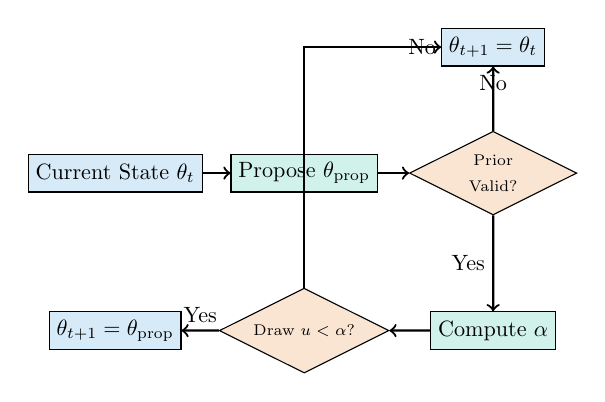
\begin{tikzpicture}[scale=0.8, every node/.style={transform shape}]
    % Nodes
    \node[draw, fill=secondary!20, minimum height=0.6cm] (start) at (0, 0) {Current State $\theta_t$};
    \node[draw, fill=primary!20, minimum height=0.6cm] (prop) at (3, 0) {Propose $\theta_{\text{prop}}$};
    \node[draw, fill=accent!20, diamond, aspect=2, align=center] (prior) at (6, 0) {\scriptsize Prior \\ \scriptsize Valid?};
    \node[draw, fill=primary!20, minimum height=0.6cm] (alpha) at (6, -2.5) {Compute $\alpha$};
    \node[draw, fill=accent!20, diamond, aspect=2, align=center] (check) at (3, -2.5) {\scriptsize Draw $u < \alpha$?};
    
    \node[draw, fill=secondary!20, minimum height=0.6cm] (accept) at (0, -2.5) {$\theta_{t+1} = \theta_{\text{prop}}$};
    \node[draw, fill=secondary!20, minimum height=0.6cm] (reject) at (6, 2.0) {$\theta_{t+1} = \theta_t$};
    
    % Paths
    \draw[->, thick] (start) -- (prop);
    \draw[->, thick] (prop) -- (prior);
    \draw[->, thick] (prior) -- node[left] {Yes} (alpha);
    \draw[->, thick] (prior) -- node[above] {No} (reject);
    \draw[->, thick] (alpha) -- (check);
    \draw[->, thick] (check) -- node[above] {Yes} (accept);
    \draw[->, thick] (check) |- node[right, pos=0.85] {No} (reject);
  \end{tikzpicture}
  \vfill
\end{frame}

% Slide 15: Hand-Worked MCMC Step
\begin{frame}{Hand-Worked MCMC Step}
  Let's walk through a single MCMC parameter step:
  \begin{itemize}
    \item \textbf{Parameter:} Rate parameter $\theta$.
    \item \textbf{Priors:} Flat uniform prior over $[0, 5]$.
    \item \textbf{Current State ($t$):} $\theta_t = 1.0$, with joint numerator score:
      $$P(D \mid \theta_t) P(\theta_t) = 0.040$$
    \item \textbf{Step 1: Propose candidate $\theta_{\text{prop}}$:}
      Draw a step from proposal distribution $\mathcal{N}(1.0, 0.05^2)$, yielding:
      $$\theta_{\text{prop}} = 1.08$$
      Check prior: $1.08 \in [0, 5]$, so the proposal is valid.
    \item \textbf{Step 2: Calculate target score at proposal:}
      $$P(D \mid \theta_{\text{prop}}) P(\theta_{\text{prop}}) = 0.032$$
    \item \textbf{Step 3: Compute acceptance probability $\alpha$:}
      $$\alpha = \min\left(1, \frac{0.032}{0.040}\right) = \min(1, 0.80) = 0.80$$
    \item \textbf{Step 4: Draw random variable $u \sim \mathcal{U}(0, 1)$:}
      \begin{itemize}
        \item If we draw $u = 0.54 \implies 0.54 < 0.80 \implies$ \textbf{Accept:} $\theta_{t+1} = 1.08$.
        \item If we draw $u = 0.87 \implies 0.87 \ge 0.80 \implies$ \textbf{Reject:} $\theta_{t+1} = 1.00$.
      \end{itemize}
  \end{itemize}
\end{frame}

% Slide 16: MCMC Diagnostics: Burn-in and Autocorrelation
\begin{frame}{MCMC Diagnostics: Burn-in and Autocorrelation}
  Before analyzing our MCMC samples, we must apply two preprocessing steps:
  \begin{description}
    \item[1. Burn-In Phase:]
      The starting point $\theta_0$ is often in a low-probability region. The early iterations show a systematic drift as the chain climbs toward the high-probability peak.
      \begin{itemize}
        \item \textbf{Action:} Discard the first $10\% - 20\%$ of the chain (e.g., discard the first 1,000 steps of a 6,000-step chain). This ensures our analyzed samples only come from the converged stationary distribution.
      \end{itemize}
    \item[2. Autocorrelation (Thinning):]
      Because MCMC states depend on preceding steps, adjacent samples are correlated.
      \begin{itemize}
        \item \textbf{Thinning:} We save only every $k$-th sample (e.g., keep every 5th or 10th sample) to reduce correlation and storage size, yielding independent draws from the posterior.
      \end{itemize}
  \end{description}
\end{frame}

% Slide 17: Trace Plots: Monitoring Convergence
\begin{frame}{Trace Plots: Monitoring Convergence}
  A **Trace Plot** displays the parameter value on the y-axis against the iteration step index on the x-axis. It is the primary diagnostic tool for monitoring chain convergence:
  \begin{itemize}
    \item \textbf{Caterpillar Look:} A healthy, converged MCMC chain looks like a tight, horizontal ``fuzzy caterpillar.'' It oscillates rapidly around a stable mean value.
    \item \textbf{Poor Mixing (Drifting):} If the chain shows long-term trends or slow waves, it has poor mixing. This means the step size is too small or the sampler is stuck in a local region.
    \item \textbf{Tuning Proposal Width ($\sigma$):}
      \begin{itemize}
        \item **Too Small:** Chain accepts almost every step but moves very slowly, failing to explore the parameter space.
        \item **Too Large:** Chain proposes massive jumps into low-probability regions, resulting in almost all steps being rejected (chain gets stuck in horizontal lines).
        \item **Optimal:** Aim for an acceptance rate of $\sim 20\% - 50\%$.
      \end{itemize}
  \end{itemize}
\end{frame}

% Slide 18: Trace Plot Configurations
\begin{frame}{Trace Plot Configurations}
  Below is a conceptual visualization of trace plots under different proposal widths:
  \begin{columns}
    \begin{column}{0.33\textwidth}
      \centering
      \alert{\textbf{Step Size Too Small}}
      \begin{tikzpicture}[scale=0.45]
        \draw[->] (0,0) -- (5,0) node[right] {Iter};
        \draw[->] (0,0) -- (0,5) node[above] {$\theta$};
        \draw[thick, primary] (0,1) -- (1,1.2) -- (2,1.5) -- (3,1.9) -- (4,2.2) -- (5,2.4);
      \end{tikzpicture}
      \scriptsize High acceptance, but slow drift. Fails to explore.
    \end{column}
    \begin{column}{0.33\textwidth}
      \centering
      \alert{\textbf{Step Size Too Large}}
      \begin{tikzpicture}[scale=0.45]
        \draw[->] (0,0) -- (5,0) node[right] {Iter};
        \draw[->] (0,0) -- (0,5) node[above] {$\theta$};
        \draw[thick, accent] (0,2) -- (1,2) -- (2,2) -- (3,2) -- (4,4.2) -- (5,4.2);
      \end{tikzpicture}
      \scriptsize High rejection rate. Long horizontal periods.
    \end{column}
    \begin{column}{0.33\textwidth}
      \centering
      \alert{\textbf{Optimal step size}}
      \begin{tikzpicture}[scale=0.45]
        \draw[->] (0,0) -- (5,0) node[right] {Iter};
        \draw[->] (0,0) -- (0,5) node[above] {$\theta$};
        \draw[thick, secondary] (0,2) -- (0.8,3) -- (1.6,1.8) -- (2.4,2.8) -- (3.2,2.1) -- (4,2.9) -- (5,2);
      \end{tikzpicture}
      \scriptsize Rapid oscillations around the mean. Healthy mixing.
    \end{column}
  \end{columns}
\end{frame}

% Slide 19: Visualizing Posterior Marginals: Corner Plots
\begin{frame}{Visualizing Posterior Marginals: Corner Plots}
  For multi-parameter models (like Type Ia coefficients $A$ and $B$), we display MCMC results using a \textbf{Corner Plot}:
  \begin{itemize}
    \item \textbf{Diagonal Panels:} 1D histograms showing the marginal posterior distribution for each parameter. The peak represents the best fit, and the width represents the uncertainty.
    \item \textbf{Off-Diagonal Panels:} 2D contour maps or scatter plots showing the joint distribution of parameter pairs.
    \item \textbf{Mapping Degeneracies:}
      If two parameters are uncorrelated, the 2D contour is circular. If they are correlated, the contour is elongated (a degeneracy diagonal).
    \item The MCMC corner plot reveals how parameters trade off against each other, exposing degeneracies that point estimates (MLE) completely hide.
  \end{itemize}
\end{frame}

% Part 3 Header
\begin{frame}[plain]
  \vfill
  \centering
  \begin{beamercolorbox}[sep=8pt,center,shadow=true,rounded=true]{palette primary}
    \usebeamerfont{title}\textbf{Part 3: Physics-Informed Machine Learning (PIML)}
  \end{beamercolorbox}
  \vfill
\end{frame}

% Slide 21: The Limits of Pure Machine Learning
\begin{frame}{The Limits of Pure Machine Learning}
  Standard machine learning models (like multi-layer perceptrons, decision trees, or random forests) are purely data-driven. They excel at finding correlations, but fail in physical sciences due to key limitations:
  \begin{description}
    \item[1. Physical Violations:] Data-driven models do not respect physical laws. A standard classifier might predict negative probabilities, violate conservation of energy, or output non-zero rates for mathematically impossible conditions.
    \item[2. Out-of-Distribution Failure:] Deep neural networks are excellent interpolators but poor extrapolators. If tested outside the boundaries of the training set, their predictions decay rapidly into unphysical regimes.
    \item[3. Massive Data Requirements:] Purely data-driven models require large training datasets to learn simple relationships (like $1/r^2$ gravity fields), which is problematic for rare astrophysical transients.
    \item[4. Lack of Physical Interpretability:] Black-box models only yield relative feature sensitivities, not physical parameters, units, or rate coefficients.
  \end{description}
\end{frame}

% Slide 22: What is Physics-Informed Machine Learning?
\begin{frame}{What is Physics-Informed Machine Learning?}
  \textbf{Physics-Informed Machine Learning (PIML)} blends empirical observations (data) with prior scientific knowledge (theoretical models, symmetries, boundary conditions, or differential equations).
  \begin{center}
    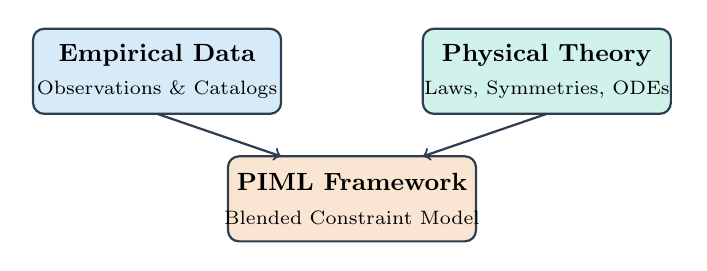
\begin{tikzpicture}[scale=0.9]
      \draw[draw=darkbg, fill=secondary!20, thick, rounded corners] (0,0) rectangle (3.5, 1.2);
      \node[align=center] at (1.75, 0.6) {\small \textbf{Empirical Data} \\ \scriptsize Observations \& Catalogs};
      
      \draw[draw=darkbg, fill=primary!20, thick, rounded corners] (5.5,0) rectangle (9, 1.2);
      \node[align=center] at (7.25, 0.6) {\small \textbf{Physical Theory} \\ \scriptsize Laws, Symmetries, ODEs};
      
      \draw[draw=darkbg, fill=accent!20, thick, rounded corners] (2.75,-1.8) rectangle (6.25, -0.6);
      \node[align=center] at (4.5, -1.2) {\small \textbf{PIML Framework} \\ \scriptsize Blended Constraint Model};
      
      \draw[thick, ->, draw=darkbg] (1.75, 0) -- (3.5, -0.6);
      \draw[thick, ->, draw=darkbg] (7.25, 0) -- (5.5, -0.6);
    \end{tikzpicture}
  \end{center}
  By constraining the search space of the model to only include physically valid functions, PIML:
  \begin{itemize}
    \item Restricts models to physically realistic boundaries.
    \item Reduces the volume of training data required by orders of magnitude.
    \item Generalizes and extrapolates reliably outside training regions.
  \end{itemize}
\end{frame}

% Slide 23: Soft Constraints: Loss-Function Regularization
\begin{frame}{Soft Constraints: Loss-Function Regularization}
  Consider a system governed by a differential equation:
  $$f(\mathbf{x}, u(\mathbf{x})) = 0$$
  where $u(\mathbf{x})$ is the physical quantity we wish to model, and $\mathbf{x}$ are inputs.
  \begin{block}{Composite Loss Function}
    To enforce this law, we define a composite loss:
    $$\mathcal{L} = \mathcal{L}_{\text{data}} + \lambda \cdot \mathcal{L}_{\text{physics}}$$
    \begin{align*}
      \mathcal{L}_{\text{data}} &= \frac{1}{N_d} \sum_{i=1}^{N_d} \|u(\mathbf{x}_i) - u_{\text{observed}, i}\|^2 \\
      \mathcal{L}_{\text{physics}} &= \frac{1}{N_{\text{col}}} \sum_{j=1}^{N_{\text{col}}} \|f(\mathbf{x}_j, u(\mathbf{x}_j))\|^2
    \end{align+1}
  \end{block}
  The regularization coefficient $\lambda > 0$ balances data matching and physics compliance. This constraint is \textbf{soft} because the optimizer might accept small physical violations to better fit noisy training data.
\end{frame}

% Slide 24: Hard Constraints: Architectural Integration
\begin{frame}{Hard Constraints: Architectural Integration}
  Soft constraints can still violate physical boundaries if the loss optimization converges to a local minimum. To ensure physical laws are met exactly, we build them directly into the network architecture:
  \begin{block}{Examples of Architectural Integration}
    \begin{itemize}
      \item \textbf{Non-Negativity Constraints:} If a physical quantity (like mass or rate) must be strictly non-negative, we pass the network's raw outputs through an exponential function:
        $$u_{\text{physical}} = e^{u_{\text{raw}}} \quad \implies \quad u_{\text{physical}} > 0 \text{ always}$$
      \item \textbf{Probability Conservation:} Enforces that predicted class assignments sum to $1.0$ by applying a Softmax layer at the final output:
        $$\sum_c P_c = 1.0 \text{ always}$$
      \item \textbf{Energy Conservation:} Hard-code an energy conservation block $E_{\text{kinetic}} + E_{\text{potential}} = E_{\text{total}}$ as an analytical layer.
    \end{itemize}
  \end{block}
\end{frame}

% Slide 25: Feature-Level Symmetries
\begin{frame}{Feature-Level Symmetries}
  We can also inject physical theory into machine learning models at the feature level:
  \begin{description}
    \item[Feature-Level (Input Integration):]
      Transform input features to satisfy symmetries and physical invariances.
      \begin{itemize}
        \item \textbf{Example:} Enforce rotational invariance by converting Cartesian coordinates $(x, y, z)$ to spherical coordinates $(r, \theta, \phi)$ before training.
      \end{itemize}
  \end{description}
\end{frame}

% Slide 26: Automatic Differentiation (Autograd) in PIML
\begin{frame}{Automatic Differentiation (Autograd) in PIML}
  To evaluate differential equations (like $\frac{du}{dx}$) in a loss-level constraint, we must calculate the derivatives of our neural network's predictions with respect to its inputs.
  \begin{itemize}
    \item \textbf{Why not numerical differentiation?}
      Finite difference approximations ($\frac{u(x+\Delta x) - u(x)}{\Delta x}$) are computationally expensive (scale poorly with input dimension) and suffer from numerical truncation errors.
    \item \textbf{Why not analytical differentiation?}
      Calculating derivatives by hand for deep, non-linear networks is highly complex and impractical.
    \item \textbf{The PIML Solution: Autograd}
      Automatic differentiation tracks operations on a computational graph. It computes exact, analytical derivatives down to machine precision using the chain rule, scaling efficiently to high dimensions.
  \end{itemize}
\end{frame}

% Slide 27: Autograd Computational Flow
\begin{frame}{Autograd Computational Flow}
  Below is a schematic showing how automatic differentiation propagates gradients through a physical loss loop. Autograd calculates the exact physical derivative $\frac{du}{dx}$ and uses it to update the model weights $W$:
  \vfill
  \centering
  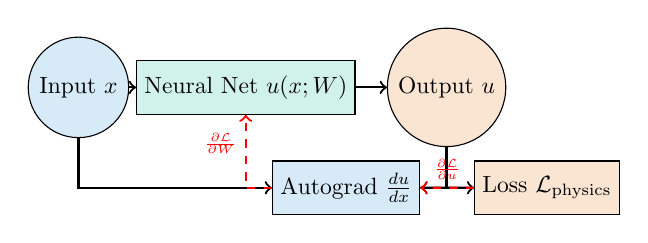
\begin{tikzpicture}[scale=0.85, every node/.style={transform shape}]
    % Graph nodes
    \node[circle, draw, fill=secondary!20] (input) at (0,0) {Input $x$};
    \node[draw, fill=primary!20, minimum height=0.8cm, minimum width=1.5cm] (nn) at (2.5,0) {Neural Net $u(x; W)$};
    \node[circle, draw, fill=accent!20] (output) at (5.5,0) {Output $u$};
    
    \node[draw, fill=secondary!20, minimum height=0.8cm, minimum width=1.5cm] (deriv) at (4,-1.5) {Autograd $\frac{du}{dx}$};
    \node[draw, fill=accent!20, minimum height=0.8cm] (loss) at (7,-1.5) {Loss $\mathcal{L}_{\text{physics}}$};
    
    % Forward paths
    \draw[->, thick] (input) -- (nn);
    \draw[->, thick] (nn) -- (output);
    \draw[->, thick] (output) |- (deriv);
    \draw[->, thick] (input) |- (deriv);
    \draw[->, thick] (deriv) -- (loss);
    
    % Backward gradient path
    \draw[->, dashed, red, thick] (loss) -- node[above] {\scriptsize $\frac{\partial \mathcal{L}}{\partial u}$} (deriv);
    \draw[->, dashed, red, thick] (deriv) -| node[left, pos=0.8] {\scriptsize $\frac{\partial \mathcal{L}}{\partial W}$} (nn);
  \end{tikzpicture}
  \vfill
\end{frame}

% Part 4 Header
\begin{frame}[plain]
  \vfill
  \centering
  \begin{beamercolorbox}[sep=8pt,center,shadow=true,rounded=true]{palette primary}
    \usebeamerfont{title}\textbf{Part 4: Case Study: Supernova Rate Modeling (Task 13)}
  \end{beamercolorbox}
  \vfill
\end{frame}

% Slide 29: The Physics of Supernova Rates
\begin{frame}{The Physics of Supernova Rates}
  In previous tasks, we compared host galaxy properties with background populations using statistical tests. Now, we define three competing models for supernova rates as functions of host galaxy properties:
  \begin{description}
    \item[1. Null (Random) Model:] Supernovae are random events that do not depend on host properties:
      $$R_{\text{Null}} = \text{const}$$
    \item[2. Core-Collapse Supernova (CC-SN) Model:] Tracks instantaneous star formation as a power law of the Star Formation Rate (SFR):
      $$R_{\text{CC}}(\text{SFR}) = \text{SFR}^\beta$$
      where $\beta \approx 1.0$ if the rate is directly proportional to the active star formation.
    \item[3. Type Ia Supernova Model:] The standard ``A+B'' model with delayed (stellar mass) and prompt (recent star formation) components:
      $$R_{\text{Ia}}(M_\star, \text{SFR}) = A \cdot \left(\frac{M_\star}{10^{10} M_\odot}\right) + B \cdot \left(\frac{\text{SFR}}{M_\odot \text{ yr}^{-1}}\right)$$
      To simplify calculations and ensure numerical stability, we define:
      $$R_{\text{Ia}}(M_\star, \text{SFR}) = A \cdot M_{\star, 10} + B \cdot \text{SFR}$$
  \end{description}
\end{frame}

% Slide 30: Formulating the Rate Likelihood
\begin{frame}{Formulating the Rate Likelihood}
  The probability of a specific galaxy $i$ hosting a supernova out of a population of $N$ galaxies is proportional to its relative rate:
  $$P(\text{host}_i \mid \theta) = \frac{R_i(\theta)}{\sum_{j=1}^N R_j(\theta)}$$
  For a sample of observed host galaxies, the joint likelihood is the product of their individual probabilities.
  \begin{block}{Negative Log-Likelihood (NLL) Formulation}
    To find the optimal parameters $\theta$, we minimize the Negative Log-Likelihood ($\mathcal{L}$):
    \begin{align*}
      \mathcal{L}(\theta) &= - \ln \prod_{i \in \text{observed}} P(\text{host}_i \mid \theta) \\
      &= - \sum_{i \in \text{observed}} \ln \left( \frac{R_i(\theta)}{\sum_{j \in \text{background}} R_j(\theta)} \right) \\
      &= -\sum_{i \in \text{observed}} \ln R_i(\theta) + N_{\text{observed}} \cdot \ln \left(\sum_{j \in \text{background}} R_j(\theta)\right)
    \end{align*}
  \end{block}
\end{frame}

% Slide 31: Classical MLE point estimation
\begin{frame}{Classical MLE point estimation}
  To fit our physical parameters ($\beta$ for CC-SNe; $A, B$ for Type Ia SNe) using point-estimate optimization:
  \begin{itemize}
    \item \textbf{Data Extraction:} Compile the observed host parameters ($M_\star, \text{SFR}$) and the background field galaxy parameters from the detected catalog.
    \item \textbf{L-BFGS-B Optimization:} Pass the custom NLL functions to a bounded minimizer (e.g., \texttt{scipy.optimize.minimize}).
    \item \textbf{Boundary Constraints:}
      \begin{itemize}
        \item Enforce parameter bounds: $\beta \in [0.1, 3.0]$ to prevent physical collapse.
        \item Enforce non-negativity: $A, B \in [0.0, 5.0]$ since supernova rates cannot be negative.
      \end{itemize}
    \item \textbf{Output Estimates:} Recover point estimates, showing that CC-SNe trace SFR ($\beta \approx 1.0$), and Type Ia SNe depend on both mass and star formation ($A, B > 0$).
  \end{itemize}
\end{frame}

% Slide 32: Constrained PINN Rate Model
\begin{frame}{Constrained PINN Rate Model}
  Instead of classical numerical solvers, we can recover parameters using a PyTorch neural network that incorporates our physical rate equations:
  \begin{itemize}
    \item \textbf{Constraining Parameters:} We define parameters ($\beta, A, B$) as neural network weights. To enforce strict positive boundaries ($A, B, \beta > 0$) without coordinate clipping, we parameterize their raw inputs and apply an exponential layer:
      $$\beta = e^{\tilde{\beta}}, \quad A = e^{\tilde{A}}, \quad B = e^{\tilde{B}}$$
    \item \textbf{Forward Propagation:} The network takes the host properties as inputs and computes the rates directly using the physical equations:
      $$R_{\text{Ia}} = A \cdot M_{\star, 10} + B \cdot \text{SFR}$$
    \item \textbf{Optimization Loss:} The model minimizes the joint Negative Log-Likelihood loss using the Adam optimizer. Gradients flow from the loss directly back to the physical weights ($\tilde{\beta}, \tilde{A}, \tilde{B}$) via automatic differentiation.
  \end{itemize}
\end{frame}

% Slide 33: PINN Rate Model Architecture
\begin{frame}{PINN Rate Model Architecture}
  Below is the network architecture for our Task 13 PINN. Unbounded parameters ($\tilde{A}, \tilde{B}$) are transformed via exponential layers to satisfy the physical positivity bounds of the rate equation:
  \vfill
  \centering
  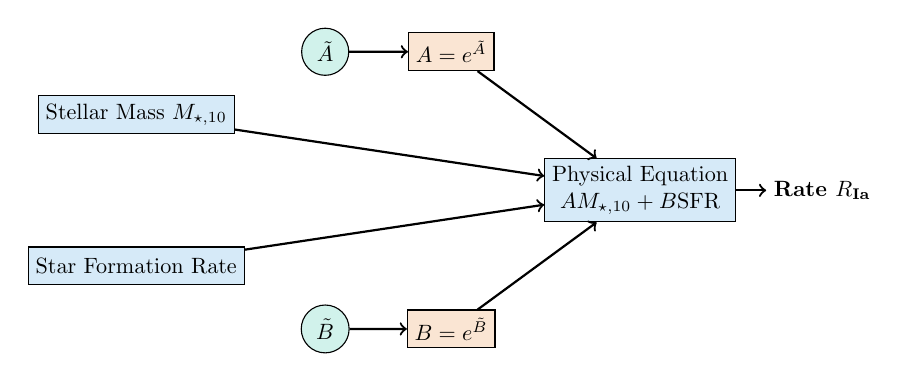
\begin{tikzpicture}[scale=0.8, every node/.style={transform shape}]
    % Inputs
    \node[draw, fill=secondary!20, minimum height=0.6cm] (mass) at (0, 1.2) {Stellar Mass $M_{\star, 10}$};
    \node[draw, fill=secondary!20, minimum height=0.6cm] (sfr) at (0, -1.2) {Star Formation Rate};
    
    % Weights
    \node[circle, draw, fill=primary!20] (a_raw) at (3, 2.2) {$\tilde{A}$};
    \node[circle, draw, fill=primary!20] (b_raw) at (3, -2.2) {$\tilde{B}$};
    
    % Exponential mapping (constraints)
    \node[draw, fill=accent!20, minimum height=0.6cm] (a_exp) at (5, 2.2) {$A = e^{\tilde{A}}$};
    \node[draw, fill=accent!20, minimum height=0.6cm] (b_exp) at (5, -2.2) {$B = e^{\tilde{B}}$};
    
    % Rate Equation node
    \node[draw, fill=secondary!20, minimum height=1cm, text width=2.8cm, align=center] (rate) at (8, 0) {Physical Equation \\ $A M_{\star, 10} + B \text{SFR}$};
    \node[right] (output) at (10, 0) {\textbf{Rate $R_{\text{Ia}}$}};
    
    % Connections
    \draw[->, thick] (a_raw) -- (a_exp);
    \draw[->, thick] (b_raw) -- (b_exp);
    \draw[->, thick] (mass) -- (rate);
    \draw[->, thick] (sfr) -- (rate);
    \draw[->, thick] (a_exp) -- (rate);
    \draw[->, thick] (b_exp) -- (rate);
    \draw[->, thick] (rate) -- (output);
  \end{tikzpicture}
  \vfill
\end{frame}

% Slide 34: Model Validation \& Goodness-of-Fit
\begin{frame}{Model Validation \& Goodness-of-Fit}
  How do we prove that our physical models are superior to the null model?
  \begin{itemize}
    \item \textbf{Synthetic Catalog Generation:}
      Using the fitted MLE parameters, we calculate rate weights $w_i = R_i / \sum R_j$ for every galaxy in the detected mock universe catalog. We sample 5,000 galaxies with replacement using these weights.
    \item \textbf{Goodness-of-Fit Testing:}
      We run 2-sample Kolmogorov-Smirnov (K-S) tests on the physical distributions of the simulated catalogs against the observed hosts:
      \begin{itemize}
        \item **Null Model Comparison:** Compares observed hosts against randomly sampled non-host galaxies. Yields $p$-values $\ll 10^{-5}$, rejecting the null hypothesis.
        \item **Physics Model Comparison:** Compares observed hosts against physics-weighted mock galaxies. Yields $p$-values $> 0.05$ (e.g., $p \approx 0.50$), confirming we cannot distinguish our model's predictions from reality.
      \end{itemize}
  \end{itemize}
\end{frame}

% Part 5 Header
\begin{frame}[plain]
  \vfill
  \centering
  \begin{beamercolorbox}[sep=8pt,center,shadow=true,rounded=true]{palette primary}
    \usebeamerfont{title}\textbf{Part 5: Case Study: Convolved DTD Solvers (Task 15)}
  \end{beamercolorbox}
  \vfill
\end{frame}

% Slide 36: The Physics of Type Ia Supernovae
\begin{frame}{The Physics of Type Ia Supernovae}
  Type Ia supernovae originate from binary systems where a carbon-oxygen white dwarf reaches the Chandrasekhar mass limit or undergoes a double white dwarf merger.
  \begin{itemize}
    \item \textbf{Delay Time ($\tau$):} The time elapsed between the formation of the star system (starburst) and the subsequent supernova explosion.
    \item \textbf{Delay Time Distribution ($\Psi(\tau)$):} The distribution of delay times for a single-burst stellar population.
    \item \textbf{Progenitor Power Law:} Theoretical white-dwarf merger models suggest that the DTD follows a power law:
      $$\Psi(\tau) \propto \tau^{-\gamma}$$
      where $\gamma \approx 1.0 - 1.2$ for delay times $\tau \ge t_{\text{min}} \approx 100\text{ Myr}$.
  \end{itemize}
\end{frame}

% Slide 37: Convolutions with Star Formation History (SFH)
\begin{frame}{Convolutions with Star Formation History (SFH)}
  A real galaxy is not a single stellar population. It forms stars continuously over cosmic time.
  \begin{block}{Convolved Rate Model}
    The supernova rate in a galaxy at age $t$ is the convolution of its historical Star Formation History ($\text{SFR}(t)$) with the DTD ($\Psi$):
    $$R_{\text{Ia}}(t) = \int_0^t \text{SFR}(t - \tau) \Psi(\tau) d\tau = \int_0^t \text{SFR}(t - \tau) \tau^{-\gamma} d\tau$$
  \end{block}
  \begin{block}{Analytical Star Formation History Model}
    We approximate the SFH using a standard delayed-exponential model:
    $$\text{SFR}(t \mid \tau_{\text{SF}}) = \text{SFR}_0 \cdot \frac{t}{\tau_{\text{SF}}} e^{-t/\tau_{\text{SF}}}$$
    where $\tau_{\text{SF}}$ is the characteristic star formation timescale.
  \end{block}
\end{frame}

% Slide 38: Discretizing the Convolution Integral
\begin{frame}{Discretizing the Convolution Integral}
  To evaluate convolved rates numerically, we map each galaxy to a cosmic time grid $t_k = k \cdot \Delta t$ from $t=0$ to the galaxy's age $T \approx 13.7\text{ Gyr}$:
  \begin{block}{Discretized Rate Equation}
    $$R_{\text{Ia}}(T \mid \tau_{\text{SF}}, \gamma) = \sum_{\tau_k \ge t_{\text{min}}}^{T} \text{SFR}(T - \tau_k \mid \tau_{\text{SF}}) \cdot \tau_k^{-\gamma} \cdot \Delta t$$
  \end{block}
  \begin{itemize}
    \item We define the delay time grid step $\Delta t = 0.1\text{ Gyr}$.
    \item $\text{SFR}(T - \tau_k \mid \tau_{\text{SF}})$ represents the star formation rate of the galaxy at the lookback time $\tau_k$.
    \item $\tau_k^{-\gamma}$ represents the fraction of stars born at lookback time $\tau_k$ that explode today.
    \item The total rate is the sum over all lookback time steps.
  \end{itemize}
\end{frame}

% Slide 39: Reconstructing $\gamma$ via PyTorch Optimization
\begin{frame}{Reconstructing $\gamma$ via PyTorch Optimization}
  We recover the power-law slope $\gamma$ from a sample of observed hosts by optimizing a PyTorch convolved rate solver:
  \begin{itemize}
    \item \textbf{Parameterization:} Define $\gamma$ as an exponential parameter to enforce physical boundaries: $\gamma = e^{\tilde{\gamma}}$.
    \item \textbf{PyTorch Solver:} Evaluates the vectorized numerical convolution across the training galaxies:
      \begin{enumerate}
        \item Computes the $\text{SFR}$ grid matrix for all galaxies based on their age and $\tau_{\text{SF}}$.
        \item Computes the DTD vector $\boldsymbol{\psi}(\gamma) = \tau^{-\gamma}$.
        \item Performs matrix multiplication to evaluate rates: $\mathbf{r} = \mathbf{S} \boldsymbol{\psi} \cdot \Delta t$.
      \end{enumerate}
    \item \textbf{Loss Function Optimization:} Minimizes the Negative Log-Likelihood:
      $$\mathcal{L} = -\sum_{i \in \text{hosts}} \ln R_i + N_{\text{hosts}} \ln \left( \sum_{j \in \text{all}} R_j \right)$$
      using the Adam optimizer. The solver successfully recovers the true power-law slope $\gamma \approx 1.15$.
  \end{itemize}
\end{frame}

% Slide 40: Convolved DTD Solver Flowchart
\begin{frame}{Convolved DTD Solver Flowchart}
  Below is the computational pipeline of our convolved solver. Gradients flow from the loss function through the numerical convolution block back to the physical parameter $\gamma$:
  \vfill
  \centering
  \begin{tikzpicture}[scale=0.85, every node/.style={transform shape}]
    % Inputs
    \node[draw, fill=secondary!20, minimum height=0.8cm, text width=2cm, align=center] (sfh) at (0, 1.2) {Galaxy SFHs \\ Matrix $\mathbf{S}$};
    \node[circle, draw, fill=primary!20] (gamma) at (0, -1.2) {$\gamma$};
    
    % DTD block
    \node[draw, fill=accent!20, minimum height=0.8cm, text width=2cm, align=center] (dtd) at (2.8, -1.2) {DTD Vector \\ $\boldsymbol{\psi}(\gamma) = \tau^{-\gamma}$};
    
    % Convolution Block
    \node[draw, fill=secondary!20, minimum height=1.2cm, text width=2.5cm, align=center] (conv) at (6, 0) {Convolution \\ $\mathbf{r} = \mathbf{S} \boldsymbol{\psi} \cdot \Delta t$};
    
    % Loss
    \node[draw, fill=accent!20, minimum height=0.8cm] (loss) at (9, 0) {NLL Loss $\mathcal{L}$};
    
    % Connections
    \draw[->, thick] (sfh) -| (conv);
    \draw[->, thick] (gamma) -- (dtd);
    \draw[->, thick] (dtd) -| (conv);
    \draw[->, thick] (conv) -- (loss);
    
    % Backpropagation arrows
    \draw[->, dashed, red, thick] (loss) -- node[above] {\scriptsize \nabla_{\mathbf{r}}\mathcal{L}} (conv);
    \draw[->, dashed, red, thick] (conv) -| node[right, pos=0.8] {\scriptsize \nabla_{\boldsymbol{\psi}}\mathcal{L}} (dtd);
    \draw[->, dashed, red, thick] (dtd) -- node[above] {\scriptsize \frac{\partial\mathcal{L}}{\partial\gamma}} (gamma);
  \end{tikzpicture}
  \vfill
\end{frame}

% Slide 41: Diagnostics and DTD Validation Results
\begin{frame}{Diagnostics and DTD Validation Results}
  Once optimization completes, we evaluate the DTD reconstruction:
  \begin{itemize}
    \item \textbf{Parameter Convergence:} The optimizer successfully updates $\gamma$ from its initialization toward the true physical power-law slope of $\gamma = 1.15$.
    \item \textbf{DTD Visual Check:} Plotting the true DTD ($\tau^{-1.15}$) against the recovered DTD ($\tau^{-\gamma_{\text{recovered}}}$) shows excellent visual agreement across delay times $0.1 \le \tau \le 3.0\text{ Gyr}$.
    \item \textbf{Loss Convergence Curve:} The loss history displays a smooth decay curve, confirming stable optimization gradients throughout training epochs.
  \end{itemize}
\end{frame}

% Slide 42: PIML Summary & Checklist
\begin{frame}{PIML Summary \& Checklist}
  When designing Physics-Informed Machine Learning models, follow these guidelines:
  \begin{block}{PIML Design Guidelines}
    \begin{enumerate}
      \item **Identify Symmetries and Slices:** Incorporate rotational, translational, or scale invariances into feature engineering before model fitting.
      \item **Enforce Bounds Architecturally:** If parameters must be positive, use exponential layers ($e^{\theta}$) to enforce this constraint exactly.
      \item **Balance Composite Losses:** If using soft constraints, monitor the loss terms $\mathcal{L}_{\text{data}}$ and $\mathcal{L}_{\text{physics}}$ separately to ensure one does not dominate the other.
      \item **Validate Physically:** Check model predictions using independent physical criteria (e.g., K-S tests or energy conservation conservation checks).
    \end{enumerate}
  \end{block}
\end{frame}

\end{document}
